\documentclass{beamer}
\usepackage{subfiles}
\usepackage{tikz}
\usepackage{color}
\usepackage[]{algorithm2e}
\usepackage[utf8]{inputenc}
\usepackage{amsmath}
\usepackage{multicol}

\usetheme{Madrid}

\title{Digital Modulation}
\subtitle{Amplitude Shift Keying, Frequency Shift Keying}

\author{Sihat Afnan \and Farhana Khan}

\institute[BUET] 
{
	Department of Computer Science \& Engineering\\
	Bangladesh University of Engineering and Technology
}

\date{June, 2021}

\subject{Theoretical Computer Science}


\begin{document}
	
	\begin{frame}
		\titlepage
	\end{frame}
	
	%\begin{frame}
	%	\tableofcontents
	%\end{frame}
	% Farhana Start
	
	% slide 2
	\begin{frame}{Introduction}
		\setbeamercovered{dynamic}
		\begin{itemize}
			\onslide\item<1->Digital Communication
			\begin{itemize}
				\item Noise Immunity
				\item Economic $\rightarrow$ Profitable
				\item Viability of distortionless regenerative repeaters
			\end{itemize}
			
			\vspace{0.2in}
			
			\onslide\item<2->But ... digital signals cannot be directly transmitted\\
			\vspace{0.1in}
			\onslide\item<2->Solution?
			
		\end{itemize}
	\end{frame}
	
	% slide 3
	\begin{frame}{Digital Modulation}
		\setbeamercovered{dynamic}
		\begin{itemize}
			\onslide\item<1->\textbf{Digital Modulation}
			\begin{itemize}
				\item Encoding Digital information
				\item Modifying carrier wave $\rightarrow$ Amplitude, Frequency, Phase
			\end{itemize}
			
			\vspace{0.3in}
			\onslide\item<2->Methods of Digital Modulation $\rightarrow$ \textbf{ASK}, \textbf{FSK}, PSK, BPSK etc.
		\end{itemize}
	\end{frame}
	
	% slide 4
	\begin{frame}{Amplitude Shift Keying (ASK)}
		\setbeamercovered{dynamic}
		\textbf{Amplitude Shift Keying}
		\begin{itemize}
			\onslide\item<1->Simplest
			\onslide\item<2->Carrier wave
			\begin{itemize}
				\item Analog
				\item High frequency
			\end{itemize}
			\onslide\item<3->A digital signal $\rightarrow$ changes amplitude of carrier
		\end{itemize}
	\end{frame}
	
	% slide 5
	\begin{frame}{Amplitude Shift Keying (ASK)}
		\begin{figure}[h]
			\centering
			
			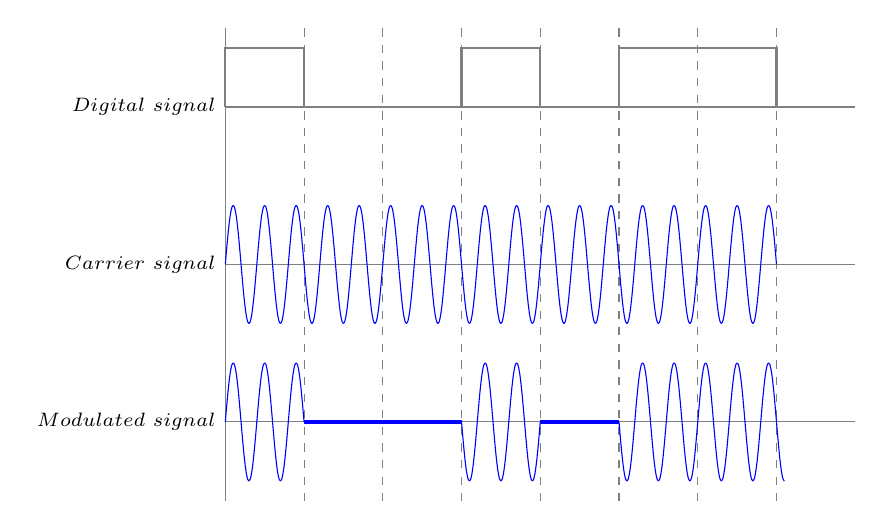
\begin{tikzpicture}
				\draw[gray] (0, 3) -- (0, -3);		% y axis
				\draw (0, 2) node[left,font=\scriptsize] {$Digital\hspace{0.1cm}signal$};
				\draw[gray]	(0, 2) -- (8, 2);		% x axis for digital signal
				\draw (0, 0) node[left,font=\scriptsize] {$Carrier\hspace{0.1cm}signal$};
				\draw[gray]	(0, 0) -- (8, 0);		% x axis for carrier signal
				\draw (0, -2) node[left,font=\scriptsize] {$Modulated\hspace{0.1cm}signal$};
				\draw[gray]	(0, -2) -- (8, -2);		% x axis for modulated signal
				
				\draw[gray, dashed, xshift=1cm] (0, 3) -- (0, -3);
				\draw[gray, dashed, xshift=2cm] (0, 3) -- (0, -3);
				\draw[gray, dashed, xshift=3cm] (0, 3) -- (0, -3);
				\draw[gray, dashed, xshift=4cm] (0, 3) -- (0, -3);
				\draw[gray, dashed, xshift=5cm] (0, 3) -- (0, -3);
				\draw[gray, dashed, xshift=6cm] (0, 3) -- (0, -3);
				\draw[gray, dashed, xshift=7cm] (0, 3) -- (0, -3);
				
				% drawing digital signal
				\draw[gray, thick] (0,2) -- (0,2.75) -- (0,2.75) -- (1,2.75) -- (1,2.75) -- (1,2);
				
				\draw[gray, thick] (1,2) -- (3,2);
				
				\draw[gray, thick] (3,2) -- (3,2.75) -- (3,2.75) -- (4,2.75) -- (4,2.75) -- (4,2);
				
				\draw[gray, thick] (4,2) -- (5,2);
				
				\draw[gray, thick] (5,2) -- (5,2.75) -- (5,2.75) -- (7,2.75) -- (7,2.75) -- (7,2);
				
				% drawing  carrier signal
				\foreach \x in {0,0.4,...,7}{
					\draw[blue] (\x,0) sin (0.1 + \x, 0.75) ;
				}
				
				\foreach \x in {0.1,0.5,...,7}{
					\draw[blue] (\x,0.75) cos (0.1 + \x, 0) ;
				}
				
				\foreach \x in {0.2,0.6,...,7}{
					\draw[blue] (\x,0) sin (0.1 + \x, -0.75) ;
				}
				
				\foreach \x in {0.3,0.7,...,7}{
					\draw[blue] (\x,-0.75) cos (0.1 + \x, 0) ;
				}
				
				% drawing  modulated signal
				\foreach \x in {0,0.4,...,1}{
					\draw[blue] (\x,-2) sin (0.1 + \x, -1.25) ;
				}
				
				\foreach \x in {0.1,0.5,...,1}{
					\draw[blue] (\x,-1.25) cos (0.1 + \x, -2);
				}
				
				\foreach \x in {0.2,0.6,...,1}{
					\draw[blue] (\x,-2) sin (0.1 + \x, -2.75) ;
				}
				
				\foreach \x in {0.3,0.7,...,1}{
					\draw[blue] (\x,-2.75) cos (0.1 + \x, -2);
				}	
				%__________
				\draw[blue, ultra thick, yshift=-4cm]  (1,2) -- (3,2);
				
				\foreach \x in {3.2,3.6,...,4}{
					\draw[blue] (\x,-2) sin (0.1 + \x, -1.25) ;
				}
				
				\foreach \x in {3.3,3.7,...,4}{
					\draw[blue] (\x,-1.25) cos (0.1 + \x, -2);
				}
				
				\foreach \x in {3,3.4,...,4}{
					\draw[blue] (\x,-2) sin (0.1 + \x, -2.75) ;
				}
				
				\foreach \x in {3.1,3.5,...,4}{
					\draw[blue] (\x,-2.75) cos (0.1 + \x, -2);
				}		
				%__________
				\draw[blue, ultra thick, yshift=-4cm] (4,2) -- (5,2);
				
				\foreach \x in {5.2,5.6,...,7}{
					\draw[blue] (\x,-2) sin (0.1 + \x, -1.25) ;
				}
				
				\foreach \x in {5.3,5.7,...,7}{
					\draw[blue] (\x,-1.25) cos (0.1 + \x, -2);
				}
				
				\foreach \x in {5,5.4,...,7}{
					\draw[blue] (\x,-2) sin (0.1 + \x, -2.75) ;
				}
				
				\foreach \x in {5.1,5.5,...,7}{
					\draw[blue] (\x,-2.75) cos (0.1 + \x, -2);
				}	
				
			\end{tikzpicture}
			
			\caption{Binary signal modulation with ASK}
		\end{figure}
	\end{frame}
	
	
	% slide 6
	\begin{frame}{Amplitude Shift Keying (ASK)}
		
		\begin{figure}[h]
			\centering
			
			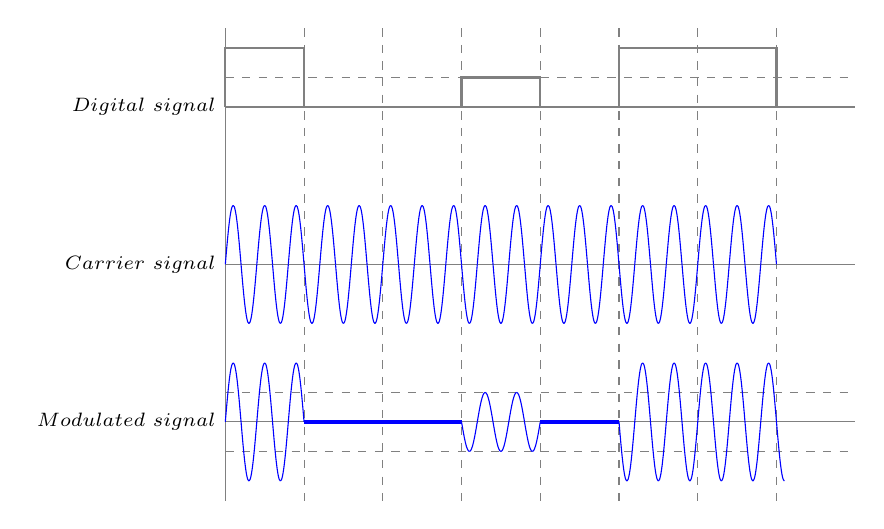
\begin{tikzpicture}
				\draw[gray] (0, 3) -- (0, -3);		% y axis
				\draw (0, 2) node[left,font=\scriptsize] {$Digital\hspace{0.1cm}signal$};
				\draw[gray]	(0, 2) -- (8, 2);		% x axis for digital signal
				\draw (0, 0) node[left,font=\scriptsize] {$Carrier\hspace{0.1cm}signal$};
				\draw[gray]	(0, 0) -- (8, 0);		% x axis for carrier signal
				\draw (0, -2) node[left,font=\scriptsize] {$Modulated\hspace{0.1cm}signal$};
				\draw[gray]	(0, -2) -- (8, -2);		% x axis for modulated signal
				
				\draw[gray, dashed, xshift=1cm] (0, 3) -- (0, -3);
				\draw[gray, dashed, xshift=2cm] (0, 3) -- (0, -3);
				\draw[gray, dashed, xshift=3cm] (0, 3) -- (0, -3);
				\draw[gray, dashed, xshift=4cm] (0, 3) -- (0, -3);
				\draw[gray, dashed, xshift=5cm] (0, 3) -- (0, -3);
				\draw[gray, dashed, xshift=6cm] (0, 3) -- (0, -3);
				\draw[gray, dashed, xshift=7cm] (0, 3) -- (0, -3);
				
				\draw[gray, dashed, yshift=2.375cm] (0, 0) -- (8, 0);
				\draw[gray, dashed, yshift=-2.375cm] (0, 0) -- (8, 0);
				\draw[gray, dashed, yshift=-1.625cm] (0, 0) -- (8, 0);
				
				% drawing digital signal
				\draw[gray, thick] (0,2) -- (0,2.75) -- (0,2.75) -- (1,2.75) -- (1,2.75) -- (1,2);
				
				\draw[gray, thick] (1,2) -- (3,2);
				
				\draw[gray, thick] (3,2) -- (3,2.375) -- (3,2.375) -- (4,2.375) -- (4,2.375) -- (4,2);
				
				\draw[gray, thick] (4,2) -- (5,2);
				
				\draw[gray, thick] (5,2) -- (5,2.75) -- (5,2.75) -- (7,2.75) -- (7,2.75) -- (7,2);
				
				% drawing  carrier signal
				\foreach \x in {0,0.4,...,7}{
					\draw[blue] (\x,0) sin (0.1 + \x, 0.75) ;
				}
				
				\foreach \x in {0.1,0.5,...,7}{
					\draw[blue] (\x,0.75) cos (0.1 + \x, 0) ;
				}
				
				\foreach \x in {0.2,0.6,...,7}{
					\draw[blue] (\x,0) sin (0.1 + \x, -0.75) ;
				}
				
				\foreach \x in {0.3,0.7,...,7}{
					\draw[blue] (\x,-0.75) cos (0.1 + \x, 0) ;
				}
				
				% drawing  modulated signal
				\foreach \x in {0,0.4,...,1}{
					\draw[blue] (\x,-2) sin (0.1 + \x, -1.25) ;
				}
				
				\foreach \x in {0.1,0.5,...,1}{
					\draw[blue] (\x,-1.25) cos (0.1 + \x, -2);
				}
				
				\foreach \x in {0.2,0.6,...,1}{
					\draw[blue] (\x,-2) sin (0.1 + \x, -2.75) ;
				}
				
				\foreach \x in {0.3,0.7,...,1}{
					\draw[blue] (\x,-2.75) cos (0.1 + \x, -2);
				}	
				%__________
				\draw[blue, ultra thick, yshift=-4cm]  (1,2) -- (3,2);
				
				\foreach \x in {3.2,3.6,...,4}{
					\draw[blue] (\x,-2) sin (0.1 + \x, -1.625) ;
				}
				
				\foreach \x in {3.3,3.7,...,4}{
					\draw[blue] (\x,-1.625) cos (0.1 + \x, -2);
				}
				
				\foreach \x in {3,3.4,...,4}{
					\draw[blue] (\x,-2) sin (0.1 + \x, -2.375) ;
				}
				
				\foreach \x in {3.1,3.5,...,4}{
					\draw[blue] (\x,-2.375) cos (0.1 + \x, -2);
				}		
				%__________
				\draw[blue, ultra thick, yshift=-4cm] (4,2) -- (5,2);
				
				\foreach \x in {5.2,5.6,...,7}{
					\draw[blue] (\x,-2) sin (0.1 + \x, -1.25) ;
				}
				
				\foreach \x in {5.3,5.7,...,7}{
					\draw[blue] (\x,-1.25) cos (0.1 + \x, -2);
				}
				
				\foreach \x in {5,5.4,...,7}{
					\draw[blue] (\x,-2) sin (0.1 + \x, -2.75) ;
				}
				
				\foreach \x in {5.1,5.5,...,7}{
					\draw[blue] (\x,-2.75) cos (0.1 + \x, -2);
				}	
				
			\end{tikzpicture}
			
			\caption{Multilevel signal modulation with ASK}
		\end{figure}
	\end{frame}
	
	% slide 7
	\begin{frame}{Amplitude Shift Keying (ASK)}
		\textbf{Demodulation of ASK}
		\begin{itemize}
			\onslide\item<1-> \textbf{Coherent Detection}
			\begin{center}
				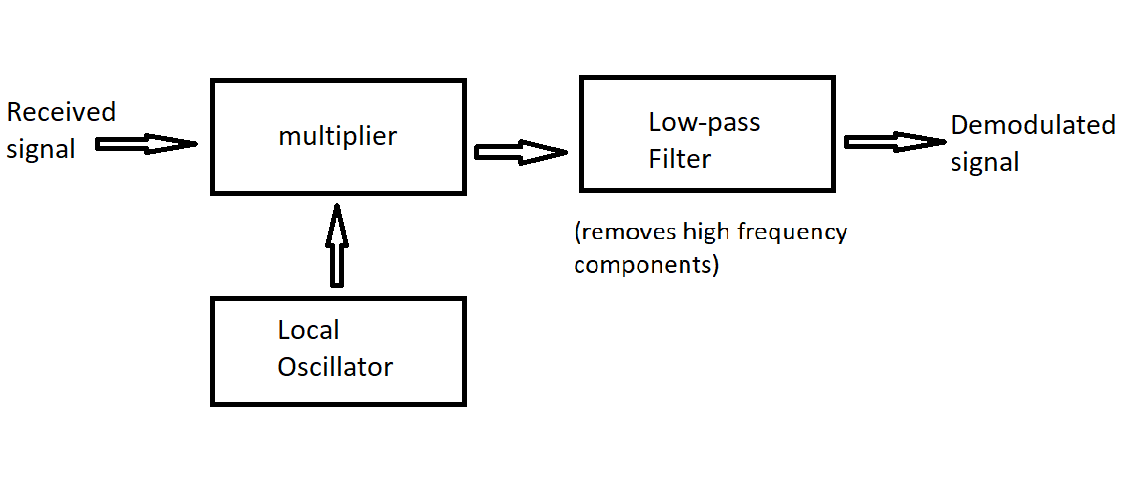
\includegraphics[scale=0.4]{synchronous_detector.png}
			\end{center}
			
			\begin{itemize}
				\onslide\item<2-> Synchronous
				\onslide\item<2-> Using Oscillator
				\onslide\item<3-> {\color{green}Efficient}
				\onslide\item<4-> {\color{red}Costly}
			\end{itemize}
		\end{itemize}
	\end{frame}
	
	
	% slide 8
	\begin{frame}{Amplitude Shift Keying (ASK)}
		\textbf{Demodulation of ASK}
		\begin{itemize}
			\onslide\item<1-> \textbf{Non coherent Detection}
			\begin{center}
				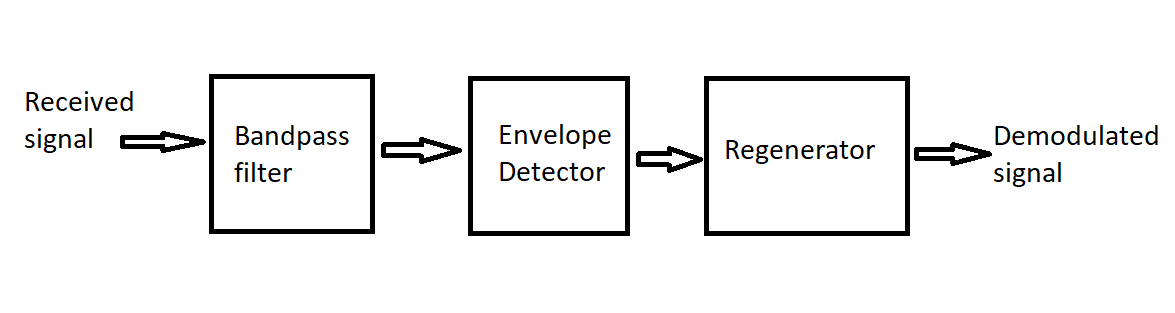
\includegraphics[scale=0.4]{asynchronous_detector.png}
			\end{center}
			
			\begin{itemize}
				\onslide\item<2-> Asynchronous
				\onslide\item<2-> Using Envelope detector  
				\onslide\item<3-> {\color{green}Less costly }
				\onslide\item<4-> {\color{red}Poor performance with less SNR}
			\end{itemize}
		\end{itemize}
	\end{frame}
	
	
	% slide 9
	\begin{frame}{Amplitude Shift Keying (ASK)}
		\begin{itemize}
			\onslide\item<1->\textbf{Applications}
			\begin{itemize}
				\onslide\item<2-> Broadcasting digital signal
				\onslide\item<3-> In optical fiber communication for LASER intensity modulation
				\onslide\item<4-> Transmit Morse codes
			\end{itemize}
		\end{itemize}
	\end{frame}
	
	% Farhana End
	
	% the rest
	\begin{frame}{Frequency Shift Keying}
		\setbeamercovered{dynamic}
		\begin{center}
			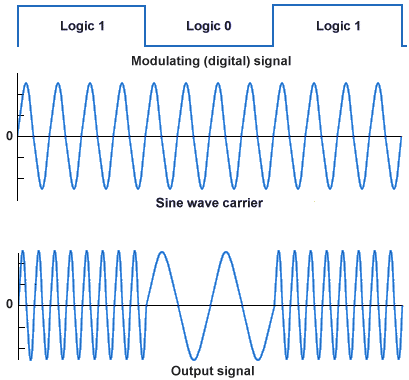
\includegraphics[scale=0.5]{2.png}
		\end{center}
		
	\end{frame}
	
	
	\begin{frame}{Frequency Shift Keying}
		\setbeamercovered{dynamic}
		\begin{enumerate}
			\onslide\item<1-> Discrete variation of carrier signal frequency. 
			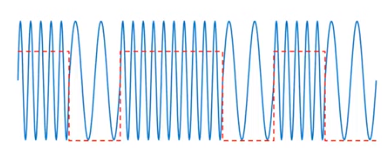
\includegraphics[height=30mm]{3.png}
			\onslide\item<2-> Different from the continuous variation of carrier signal frequency in analog FM modulation. 
			\onslide\item<3-> Number of discrete frequencies can be \\
			\begin{itemize}
				\item two : Binary FSK or BFSK
				\item More than two : M-ary FSK
			\end{itemize}  
			
		\end{enumerate}
	\end{frame}
	
	
	
	\begin{frame}{BFSK}
		\setbeamercovered{dynamic}
		\begin{enumerate}
			\onslide\item Two frequencies : Mark and Space
			\onslide\item Same amount of deviation from the carrier frequency $f_c$ 
			\vspace{1cm}                                   
			\begin{center}
				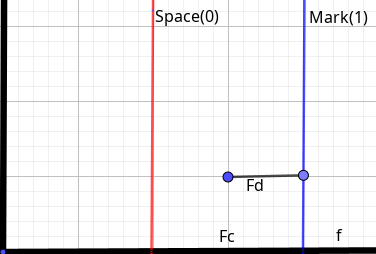
\includegraphics[scale=0.4]{11.png}
			\end{center}  
			
		\end{enumerate}
	\end{frame}
	
	
	\begin{frame}{BFSK}
		\setbeamercovered{dynamic}
		\begin{flushleft}
		\begin{enumerate}
		
		    \onslide\item<1-> Carrier amplitude doesn't change(only frequency)
		
			
			\centering
			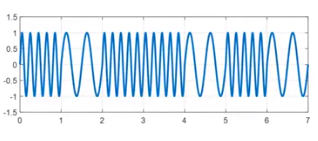
\includegraphics[scale=0.8]{7.png}
			\onslide\item<2-> Simplifies the amplifier design and selection \newline
			
		\end{enumerate}
		\end{flushleft}
	\end{frame}
	
	\begin{frame}{Tone Spacing}
		\setbeamercovered{dynamic}
		\begin{itemize}
			\onslide\item<1-> How far apart should the mark an space be?
			\begin{flushleft} 
				\begin{itemize}
					\item Too close - InterSymbol interference(ISI)
				\end{itemize}
				
			\end{flushleft}
			
			\centering
			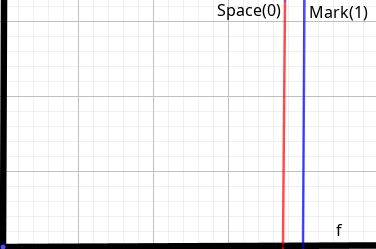
\includegraphics[scale=0.4]{13.png} 
			
			\begin{flushleft} 
				\begin{itemize}
					\onslide\item Too far - Excessive Bandwith  
				\end{itemize}
				
			\end{flushleft}
			
			\begin{center}
				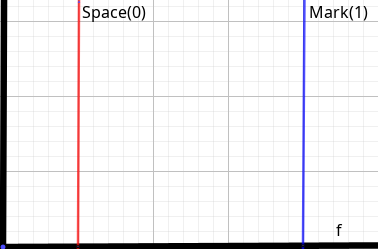
\includegraphics[scale=0.4]{12.png}
			\end{center}
			
		\end{itemize}
	\end{frame}
	
	
	\begin{frame}{Minimum FSK Bandwith}
		\setbeamercovered{dynamic}
		\begin{enumerate}
			\onslide\item<1-> Function of
			\begin{itemize}
				\item Frequency Deviation($F_d$)
				\item Bit Rate($F_b$)
			\end{itemize}
			\begin{center}
				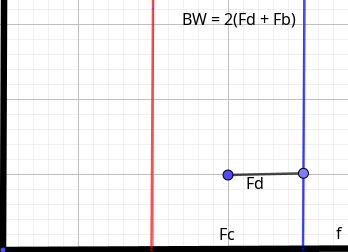
\includegraphics[scale=0.6]{14.png}
			\end{center}
			%\centering	
			\onslide\item<2-> But how far apart the tone should be?  
			
		\end{enumerate}
	\end{frame}
	
	\begin{frame}{Modulation Index}
		\setbeamercovered{dynamic}
		\begin{enumerate}
			\onslide\item<1-> Tones should be as close as possible without creating ISI.
			\onslide\item<2-> Modulation Index			
			\begin{center}
				\item $h = \frac{2*F_d}{F_b}$
				\item       
			\end{center}
			
			\onslide\item<3-> Optimal detetction occurs when h$\geq$ 1  
			\onslide\item<4-> Why MSK needs less bandwith than BFSK for a given bit rate? 
		\end{enumerate}
	\end{frame}
	
	
	\begin{frame}{MFSK}
		\setbeamercovered{dynamic}
		\begin{enumerate}
			\onslide\item<1-> More than two frequencies
			
			\begin{center}
				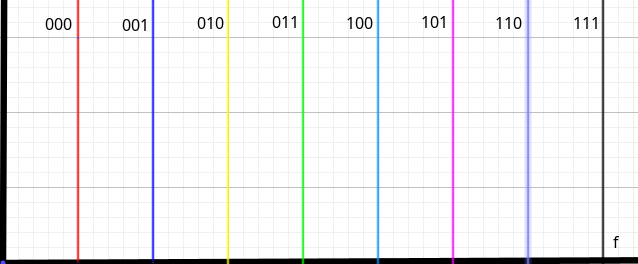
\includegraphics[scale=0.5]{mfsk.png}
			\end{center}
			\onslide\item<2-> Each MFSK tone corresponds to ${\log_2 M}$ bits
			\onslide\item<3-> BFSK Formulas are applicable for MFSK too. 
		\end{enumerate}
	\end{frame}
	
	\begin{frame}{Application of FSK}
		\setbeamercovered{dynamic}
		\begin{enumerate}
			\item $Paging (F_d\uparrow , F_b\downarrow)	$	 \\	
			\begin{center}
				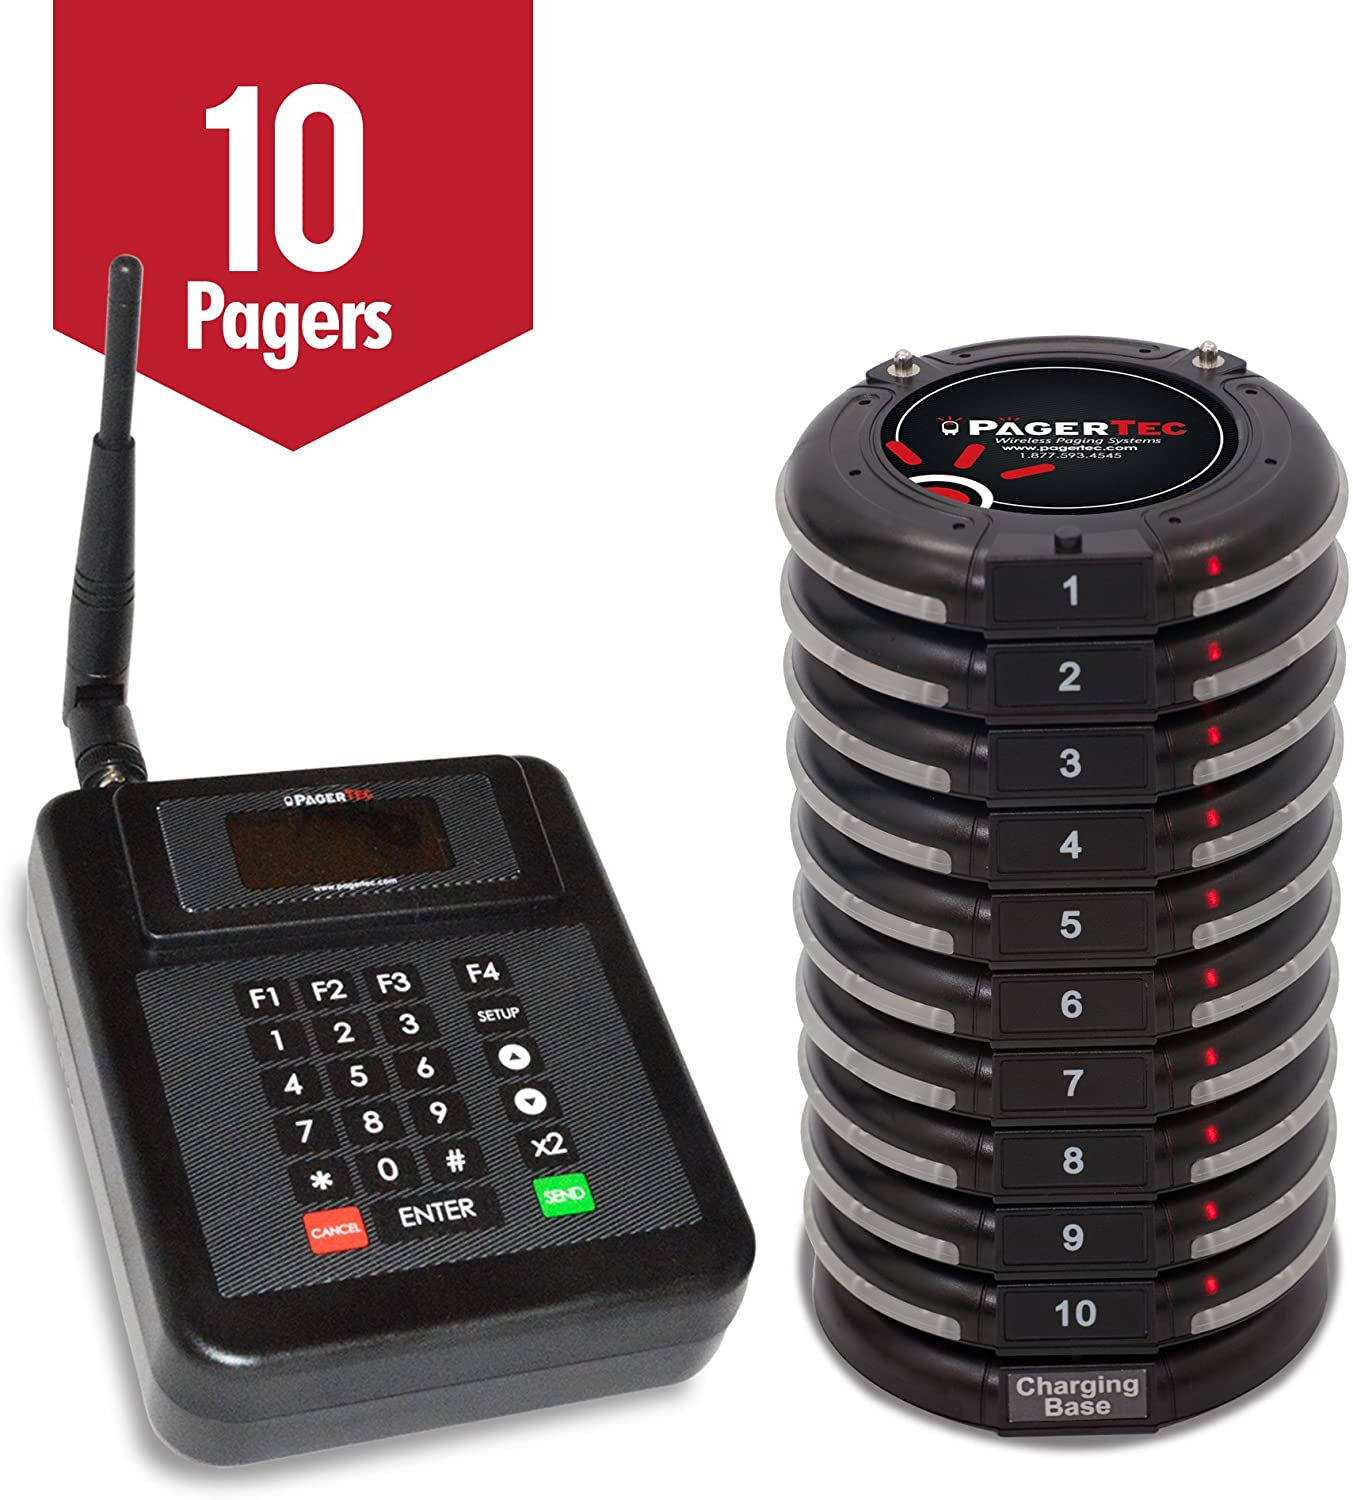
\includegraphics[scale=0.05]{paging.jpg}
			\end{center}
			
			\item Digital Radio Technology
			\item Data Collection and Remote Controls
		\end{enumerate}
	\end{frame}
	
	
	\begin{frame}{The End}
		\centering
		\Huge Thank You \\
		\Large Any Question?
	\end{frame}
	
	
\end{document}


